\documentclass[12pt,letterpaper]{exam}
\usepackage[lmargin=1in,rmargin=1in,tmargin=1in,bmargin=1in]{geometry}
\usepackage{../style/exams}

% -------------------
% Course & Exam Information
% -------------------
\newcommand{\course}{MATH 122: Exam 3}
\newcommand{\term}{Fall --- 2024}
\newcommand{\examdate}{11/21/2024}
\newcommand{\timelimit}{75 Minutes}

\setbool{hideans}{true} % Student: True; Instructor: False

% -------------------
% Content
% -------------------
\begin{document}

\examtitle
\instructions{Write your name on the appropriate line on the exam cover sheet. This exam contains \numpages\ pages (including this cover page) and \numquestions\ questions. Check that you have every page of the exam. Answer the questions in the spaces provided on the question sheets. Be sure to answer every part of each question and show all your work. If you run out of room for an answer, continue on the back of the page --- being sure to indicate the problem number.} 
\scores
\bottomline
\newpage


% -------------------
% Questions
% -------------------
\begin{questions}

% Question 1
\newpage
\question[15] Consider the plot of a function $f(x)$ given below.
	\[
	\fbox{
	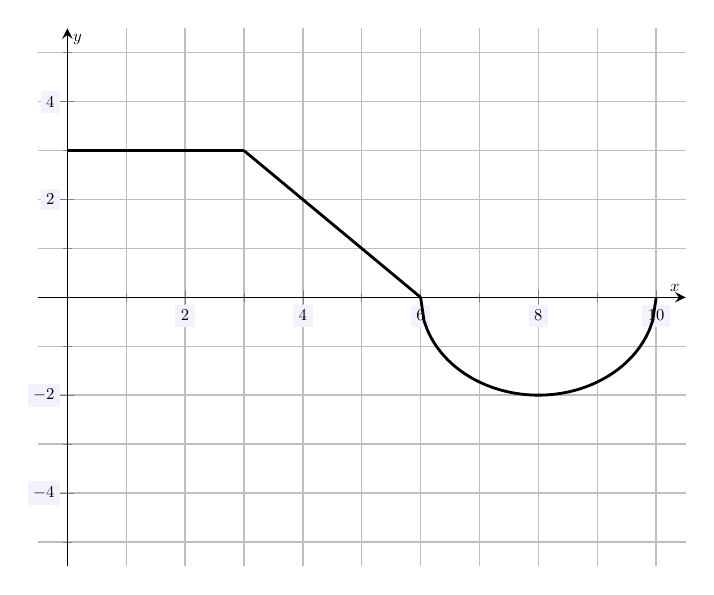
\begin{tikzpicture}[scale=1.2,every node/.style={scale=0.5}]
	\begin{axis}[
	grid=both,
	axis lines=middle,
	ticklabel style={fill=blue!5!white},
	xmin= -0.5, xmax=10.5,
	ymin= -5.5, ymax=5.5,
	xtick={-2,0,...,10},
	ytick={-6,-4,...,6},
	minor tick = {-10,-9,...,10},
	xlabel=\(x\),ylabel=\(y\),
	]
	\addplot[line width= 0.03cm,samples=5,domain= 0:3] ({x},{3});
	\addplot[line width= 0.03cm,samples=5,domain= 3:6] ({x},{6 - x});
	\addplot[line width= 0.03cm,samples=70,domain= 6:10] ({x},{-sqrt(4 - (x - 8)^2)});
	\node at (1,7.2) {$f(x)$};
	\end{axis}
	\end{tikzpicture}
	}
	\]
Using the above plot, compute the following: \par\vspace{0.3cm}
	\begin{enumerate}[(a)]
	\item $\displaystyle\int_0^3 f(x) \;dx=$ \vfill
	\item $\displaystyle\int_6^{10} f(x) \;dx=$ \vfill
	\item $\displaystyle\int_0^{10} f(x) \;dx=$ \vfill
	\item $\displaystyle\int_5^5 f(x) \;dx=$ \vfill
	\item The area between $f(x)$ and the $x$-axis. \vfill
	\end{enumerate}



% Question 2
\newpage
\question[15] A jet plane is descending for a landing. The velocity in mph at a time $t$~minutes from the start of its descent, $v(t)$, is given in the table below.
	\begin{table}[!ht]
	\centering
	\begin{tabular}{|l||c|c|c|c|c|c|c|} \hline
	Time, $t$ & 0 & 5 & 10 & 15 & 20 \\ \hline
	Velocity, $v(t)$ & 550 & 520 & 500 & 490 & 410 \\ \hline
	\end{tabular}
	\end{table}

\begin{enumerate}[(a)]
\item Using the table above and a right-hand sum, approximate $\displaystyle\int_0^{20} v(t) \;dt$ as accurately as possible. \vspace{4cm} \vfill
\item What does your value in (a) represent? \vfill
\item Based on the table is your approximation in (a) likely an under- or over-estimate? \vfill
\end{enumerate}



% Question 3
\newpage
\question Showing all your work, compute the following: \par\vspace{0.3cm}
	\begin{parts}
	\part[5] $\displaystyle\int (\sqrt{x} + e^x) \;dx$ \vfill
	\part[5] $\displaystyle\int_{-1}^1 \left( x^3 - 6x^2 \right) \;dx$ \vfill
	\part[5] $\displaystyle\int \left( 5^x - \dfrac{2}{x} \right)\;dx$ \vfill
	\end{parts}



% Question 4
\newpage
\question[10] Showing all your work, use a left-hand sum with three evenly spaced rectangles to approximate the following:
	\[
	\int_1^{13} \left( x \ln x - 1 \right) \;dx
	\]



% Question 5
\newpage
\question Showing all your work, compute the following: \par\vspace{0.3cm}
	\begin{parts}
	\part[5] $\displaystyle\int \dfrac{x^3 - 5x^2 + 6}{x^2} \;dx$ \vfill
	\part[5] $\displaystyle\int (x^4 + 3)^2 \;dx$ \vfill
	\end{parts}



% Question 6
\newpage
\question Showing all your work, use $u$-substitution to compute the following: \par\vspace{0.3cm}
	\begin{parts}
	\part[5] $\displaystyle\int x \sqrt{3x^2 + 5} \;dx$ \vfill
	\part[5] $\displaystyle\int_0^4 (5 - 2x)^3 \;dx$ \vfill
	\end{parts}



% Question 7
\newpage
\question[15] The marginal cost of producing $q$ dill pickle scented candles is given by $C'(q)= 1.5 + \dfrac{100}{2q + 1}$. The total cost to produce 6,000 candles is \$34,500. 
	\begin{enumerate}[(a)]
	\item Find the cost function, $C(q)$.
	\item What are the fixed costs?
	\item Find the cost to produce 20,000 candles?
	\end{enumerate}



% Question 8
\newpage
\question[10] A fresh brewed, decaf venti cup of coffee with 3 squirts of vanilla, 8 pumps of caramel, 5 sugars, and almond milk is at 195$^\circ$F. The rate of change in temperature of the coffee, measured in degrees Fahrenheit per minute, $t$ minutes from now is given by $r(t)= -15 e^{-0.25t}$. Estimate the coffee's temperature after 30~minutes. Be sure to show all your work.


\end{questions}
\end{document}